\chapter{Analisis}
\label{chap:analisis}

Bab ini membahas hasil analisis berdasarkan dasar teori yang sudah dijelaskan sebelumnya. Pada bab ini akan dijelaskan hasil analisis \textit{dataset} yang akan digunakan dalam pengujian, representasi dokumen dalam perangkat lunak, dan pemodelan ruang vektor pada dokumen. Selain itu pada bab ini juga akan dibahas mengenai representasi kromosom, fungsi \textit{fitness}, dan beberapa operasi genetik yang akan digunakan dalam membuat pengelompokan dokumen berbasis algoritma genetika.

\section{Analisis \textit{Dataset}}
Pada bagian ini akan dibahas mengenai \textit{dataset} yang akan digunakan dalam proses pengujian. \textit{Dataset} yang akan digunakan berisi artikel berita \textit{BBC News} dan disediakan untuk menjadi tolok ukur dalam penelitian pembelajaran mesin. Karakteristik dari \textit{dataset} ini antara lain:

\begin{itemize}
	\item Terdiri dari 2225 dokumen yang berasal dari \textit{website BBC News} dari tahun 2004-2005.
	\item Dokumen ditulis dalam Bahasa Inggris.
	\item Terbagi menjadi lima topik yaitu \textit{business, entertainment, politics, sport}, dan \textit{tech}.
	\item Pada topik \textit{business} terdapat 510 dokumen, \textit{entertainment} terdapat 386 dokumen, \textit{politics} terdapat 417 dokumen, \textit{sport} terdapat 511 dokumen, dan \textit{tech} terdapat 401 dokumen.
	\item Dokumen merupakan \textit{plain text} yang ditulis dalam file dengan ekstensi \textit{TXT}.
	\item Rata-rata dalam satu dokumen terdapat 384 kata.
\end{itemize}

\section{Representasi Dokumen}
Dokumen tidak bisa langsung digunakan begitu saja dalam proses pengelompokan. Tidak seperti manusia yang dapat melakukan proses secara manual, komputer tidak dapat menemukan nilai informasi dari data mentah berupa dokumen. Dokumen yang ada perlu direpresentasikan menjadi bentuk yang bisa diambil informasinya baru kemudian dapat diolah dalam proses lebih lanjut. Model ruang vektor (Subbab \ref{sec:vsm}) digunakan dalam penelitian ini untuk merepresentasikan dokumen sehingga informasinya dapat diproses dengan lebih mudah.

\section{Model Ruang Vektor}
\label{sec:analysis:vsm}
Pada subbab \ref{sec:vsm} telah dijelaskan bahwa dokumen akan dibentuk ke dalam sebuah vektor yang memiliki banyak dimensi berdasarkan banyaknya \term berbeda dalam dokumen. Seperti yang telah dibahas pada subbab \ref{sec:termWeight}, ada dua cara untuk menentukan bobot dari suatu \term dalam dokumen yaitu bobot frekuensi dan bobot tf-idf. Sebagai contoh akan digunakan tiga dokumen berikut:

\begin{enumerate}
	\item Penjualan properti di Indonesia meningkat di Bulan Februari.
	\item Penjualan asuransi kendaraan di Indonesia meningkat.
	\item Bulan Februari merupakan bulan puncak penjualan kendaraan.
\end{enumerate}

Berdasarkan tiga dokumen tersebut akan ditentukan bobot dari masing-masing \textit{term} dalam tiap dokumen untuk setiap jenis pembobotan.

\subsection{Bobot Frekuensi}
Pada subbab \ref{sub:freq} telah dijelaskan bahwa bobot frekuensi dari suatu \term dapat ditentukan dengan cara menghitung banyaknya kemunculan \term tersebut dalam dokumen. Hasil perhitungan bobot frekuensi berdasarkan contoh pada subbab \ref{sec:analysis:vsm} ditunjukkan dalam tabel \ref{tbl:freq}.

\begin{table}[h]
	\centering
	\begin{tabular}{|c|c|c|c|} \hline
		\multirow{2}{*}{\Term} & \multicolumn{3}{c|}{Bobot} \\ \cline{2-4}
		& Dokumen 1 & Dokumen 2 & Dokumen 3 \\ \hline 
        penjualan & 1 & 1 & 1 \\ \hline
        properti & 1 & 0 & 0 \\ \hline
        di & 2 & 1 & 0 \\ \hline
        indonesia & 1 & 1 & 0 \\ \hline
        meningkat & 1 & 1 & 0 \\ \hline
        bulan & 1 & 0 & 2 \\ \hline
        februari & 1 & 0 & 1 \\ \hline
        asuransi & 0 & 1 & 0 \\ \hline
        kendaraan & 0 & 1 & 1 \\ \hline
        merupakan & 0 & 0 & 1 \\ \hline
        puncak & 0 & 0 & 1 \\ \hline
	\end{tabular}
	\caption{Hasil perhitungan bobot frekuensi}
	\label{tbl:freq}
\end{table}

Semakin besar bobot, maka \term dianggap semakin mewakili isi dokumen. Sebagai contoh pada tabel \ref{tbl:freq}, \term "di" muncul dua kali pada dokumen 1 sehingga berbobot 2, muncul satu kali pada dokumen 2 sehingga berbobot 1, dan tidak muncul sama sekali pada dokumen 3 sehingga memiliki bobot 0 sehingga \term "di" dianggap mewakili dokumen 1 karena muncul dua kali pada dokumen tersebut.

\subsection{Bobot TF-IDF}
Berbeda dengan bobot frekuensi yang hanya menghitung frekuensi kemunculan \term pada dokumen, perhitungan bobot TF-IDF ini memerlukan perhitungan seperti yang telah dijelaskan dalam persamaan \ref{eq:tf-idf} pada subbab \ref{sub:tf-idf}. Hasil perhitungan bobot TF-IDF berdasarkan contoh pada Subbab \ref{sec:analysis:vsm} ditunjukkan dalam Tabel \ref{tbl:tf-idf}.

\begin{table}[h]
	\centering
	\begin{tabular}{|c|c|c|c|} \hline
		\multirow{2}{*}{\Term} & \multicolumn{3}{c|}{Bobot} \\ \cline{2-4}
		& Dokumen 1 & Dokumen 2 & Dokumen 3 \\ \hline 
        penjualan & 0 & 0 & 0 \\ \hline
        properti & 0.0596 & 0 & 0 \\ \hline
        di & 0.0440 & 0.0293 & 0 \\ \hline
        indonesia & 0.0220 & 0.0293 & 0 \\ \hline
        meningkat & 0.0220 & 0.0293 & 0 \\ \hline
        bulan & 0.0220 & 0 & 0.0503 \\ \hline
        februari & 0.0220 & 0 & 0.0252 \\ \hline
        asuransi & 0 & 0.0795 & 0 \\ \hline
        kendaraan & 0 & 0.0293 & 0.0252 \\ \hline
        merupakan & 0 & 0 & 0.0682 \\ \hline
        puncak & 0 & 0 & 0.0682 \\ \hline
	\end{tabular}
	\caption{Hasil perhitungan bobot TF-IDF}
	\label{tbl:tf-idf}
\end{table}

Sama halnya dengan bobot frekuensi, semakin besar bobotnya maka \term tersebut semakin mewakili isi dokumen. \Term "penjualan" muncul di ketiga dokumen sehingga pada saat perhitungan IDF menghasilkan nilai nol ($log \frac{N}{N_i}=log \frac{3}{3} = 0$). Dapat disimpulkan bahwa \term "penjualan" tidak mewakili dokumen manapun karena muncul di semua dokumen. Untuk menjelaskan nilai dalam tabel, dijelaskan  salah satu contoh perhitungan TF-IDF untuk \term "properti" pada dokumen 1 ditunjukkan dalam Persamaan \ref{eq:tf-idf-ex1} dan \ref{eq:tf-idf-ex2}.

\begin{equation}
	\label{eq:tf-idf-ex1}
	\begin{gathered}
 	tf_{i,d}=\frac{f_{i,d}}{\sum_{t \in d}f_{t,d}} \\
	tf_{"properti",1}=\frac{1}{8}=0.125 \\
	\end{gathered}
\end{equation}
	
\begin{equation}
	\label{eq:tf-idf-ex2}
	\begin{gathered}
	w_{i,d}=tf_{i,d} \times log \frac{N}{N_i} \\
	w_{"properti",1}=0.125 \times log \frac{3}{1} = 0.125 \times 0.4771 = 0.0596
	\end{gathered}
\end{equation}

\section{Representasi Kromosom}
Setiap \textit{string} kromosom merupakan deretan bilangan riil yang merepresentasikan $K$ titik pusat \textit{cluster} (\textit{centroid}) dalam bentuk vektor. Dalam ruang $N$ dimensi, panjang dari kromosom akan menjadi $N\times K$ gen. $N$ kata pertama merepresentasikan $N$ dimensi dari \textit{centroid} pertama, $N$ kata selanjutnya merepresentasikan $N$ dimensi dari \textit{centroid} kedua, dan seterusnya. Sebagai contoh apabila diketahui ada tiga buah \textit{centroid} dalam bidang dua dimensi $\mathbf{C1}$ (3.05, 1.43), $\mathbf{C2}$ (15.85, 14.23), dan $\mathbf{C3}$ (5.12, 9.45). Hasil representasi ketiga \textit{centroid} pada kromosom ditunjukkan oleh Tabel \ref{tbl:chromosome}..

\begin{table}[h]
	\centering
	\begin{tabular}{|c|c|c|c|c|c|}
		\multicolumn{2}{c}{\textbf{$\mathbf{C1}$}} & \multicolumn{2}{c}{\textbf{$\mathbf{C2}$}} & \multicolumn{2}{c}{$\mathbf{C3}$}\\ \hline
		3.05 & 1.43 & 15.85 & 14.23 & 5.12 & 9.45\\ \hline
	\end{tabular}
	\caption{Representasi \textit{centroid} ke dalam kromosom}
	\label{tbl:chromosome}
\end{table}

\section{Fungsi \textit{Fitness}}
Perhitungan \textit{fitness} dalam penelitian ini terdiri dari dua tahap. Pada tahap pertama, terjadi pembentukan \textit{cluster} berdasarkan titik pusat yang terkandung dalam kromosom. Hal ini dilakukan dengan menetapkan setiap titik $x_i,i=1,2, ... ,n$ ke dalam sebuah \textit{cluster} $C_j$ dengan \textit{centroid} $z_j$ sehingga

\begin{equation}
\Vert x_i-z_j \Vert < \Vert x_i-z_p \Vert , p=1,2, ... ,K \mbox{, dan } p \neq j.
\end{equation}

Setelah proses pengelompokan selesai, titik pusat yang terkandung dalam kromosom diganti dengan rata-rata titik dari tiap \textit{cluster}. Dengan kata lain, untuk \textit{cluster} $C_i$, \textit{centroid} baru $z_i^*$ dapat dihitung menggunakan Persamaan \ref{eq:centroid}

\begin{equation}
\label{eq:centroid}
z_i^*=\frac{1}{n_i} \sum_{x_j\in C_i} x_j,   i=1,2, ... ,K.
\end{equation}

dengan $z_i^*$ merupakan titik pusat \textit{cluster} ke-$i$, $n_i$ merupakan jumlah anggota \textit{cluster} ke-$i$, dan $x_j$ merupakan titik ke-$j$ yang merupakan anggota dari \textit{cluster} ke-$i$. $z_i^*$ ini akan menggantikan $z_i$ sebelumnya di kromosom. Ada dua metode perhitungan fungsi fitness yang diimplementasikan dalam penelitian ini yaitu \textit{cosine similarity}.

\subsection{Cosine Similarity}
Perhitungan \textit{fitness} menggunakan \textit{cosine similarity} dapat dilakukan dengan Persamaan \ref{eq:cosSim}
\begin{equation}
\label{eq:cosSim}
	\begin{gathered}
	f=\sum_{i=1}^K f_i , \\
	f_i=\sum_{x_j\in C_i}\dfrac{x_j\cdot z_i}{\parallel x_j \parallel \times \parallel z_i \parallel}
	\end{gathered}
\end{equation}

semakin besar nilai dari fungsi \textit{fitness} $f$, maka kromosom tersebut semakin mendekati solusi yang optimal.

\section{Operasi Genetik}
Ada beberapa operasi genetik yang akan dibahas, di antaranya: inisialisasi populasi, seleksi, persilangan, dan mutasi.

\subsection{Inisialisasi Populasi}
$K$ \textit{centroid} yang terkandung dalam kromosom pada mulanya dipilih secara acak sebanyak $K$ titik dari keseluruhan himpunan data. Lalu proses ini diulang sebanyak $P$ kali di mana $P$ merupakan ukuran populasi yang diinginkan.

\subsection{Seleksi}
Proses seleksi ini terjadi berdasarkan konsep \textit{survival of the fittest} yang diadaptasi dari sistem genetika alami. Konsep ini mengatakan bahwa hanya individu terbaik yang akan bertahan hidup (lolos seleksi alam). Dengan mengadaptasi konsep tersebut, GA menerapkan seleksi berdasarkan nilai \textit{fitness} tiap individu. Dalam penelitian ini, calon induk dari generasi selanjutnya dipilih dengan menggunakan teknik \textit{roulette-wheel selection}. Seperti yang telah dijelaskan dalam Subbab \ref{sub:selection}, dalam teknik \textit{roulette-wheel selection} individu yang memiliki nilai \textit{fitness} lebih tinggi akan memiliki peluang lebih besar untuk terpilih dan menjadi induk bagi generasi berikutnya. Namun karena masih ada peluang individu dengan nilai \textit{fitness} terbaik tidak terpilih, maka dalam penelitian ini juga akan digunakan teknik elitisme \cite{ahn2003elitism}. Dengan digunakannya elitisme, maka individu dengan nilai \textit{fitness} terbaik akan disalin dan langsung menjadi anggota dari generasi berikutnya. Hal ini akan menjamin individu terbaik tidak akan hilang akibat tidak terpilih oleh \textit{roulette-wheel selection}.

\subsection{Persilangan}
Persilangan dalam penelitian ini terjadi terhadap dua induk dengan satu titik potong (\textit{single-point crossover}). Misalkan kromosom memiliki panjang $l$, sebuah angka acak akan diambil sebagai titik potong dalam batas [1,$l-1$]. Bagian kromosom sebelah kanan titik potong akan ditukar  antara kedua induk sehingga menghasilkan dua individu keturunan.

\subsection{Mutasi}
Setiap kromosom mengalami mutasi dengan probabilitas mutasi tetap $\mu_c$. Apabila mutasi terjadi, maka akan ditentukan gen mana yang akan mengalami mutasi dengan mengambilnya secara acak. Nilai gen yang baru akan ditentukan dari pembangkitan suatu angka acak yang berada antara batas minimum kemunculan istilah (0) dan total kemunculan istilah tersebut dari keseluruhan dokumen. Sebagai contoh dengan menggunakan Tabel \ref{tbl:chromosome}, akan ditentukan satu dari enam gen yang akan mengalami mutasi. Misalkan dalam contoh ini gen kedua yang mengalami mutasi. Lalu akan dilakukan pembangkitan angka acak antara 0 sampai dengan total kemunculan istilah dari keseluruhan dokumen (dalam contoh ini bernilai 9). Kromosom hasil mutasi ditunjukkan dalam Tabel \ref{tbl:mutated}

\begin{table}[h]
	\centering
	\begin{tabular}{|c|c|c|c|c|c|}
		\multicolumn{2}{c}{\textbf{$\mathbf{C1}$}} & \multicolumn{2}{c}{\textbf{$\mathbf{C2}$}} & \multicolumn{2}{c}{$\mathbf{C3}$}\\ \hline
		3.05 & {\color{red} \textbf{4.18}} & 15.85 & 14.23 & 5.12 & 9.45\\ \hline
	\end{tabular}
	\caption{Kromosom hasil mutasi}
	\label{tbl:mutated}
\end{table}


%\section{Diagram Kelas}
%Berdasarkan hasil analisis dari masalah yang dihadapi, dibentuklah diagram kelas pada gambar \ref{fig:diagramkelas} sebagai gambaran dari perangkat lunak yang akan dibuat.
%
%\begin{figure}[h]
%	\begin{center}
%		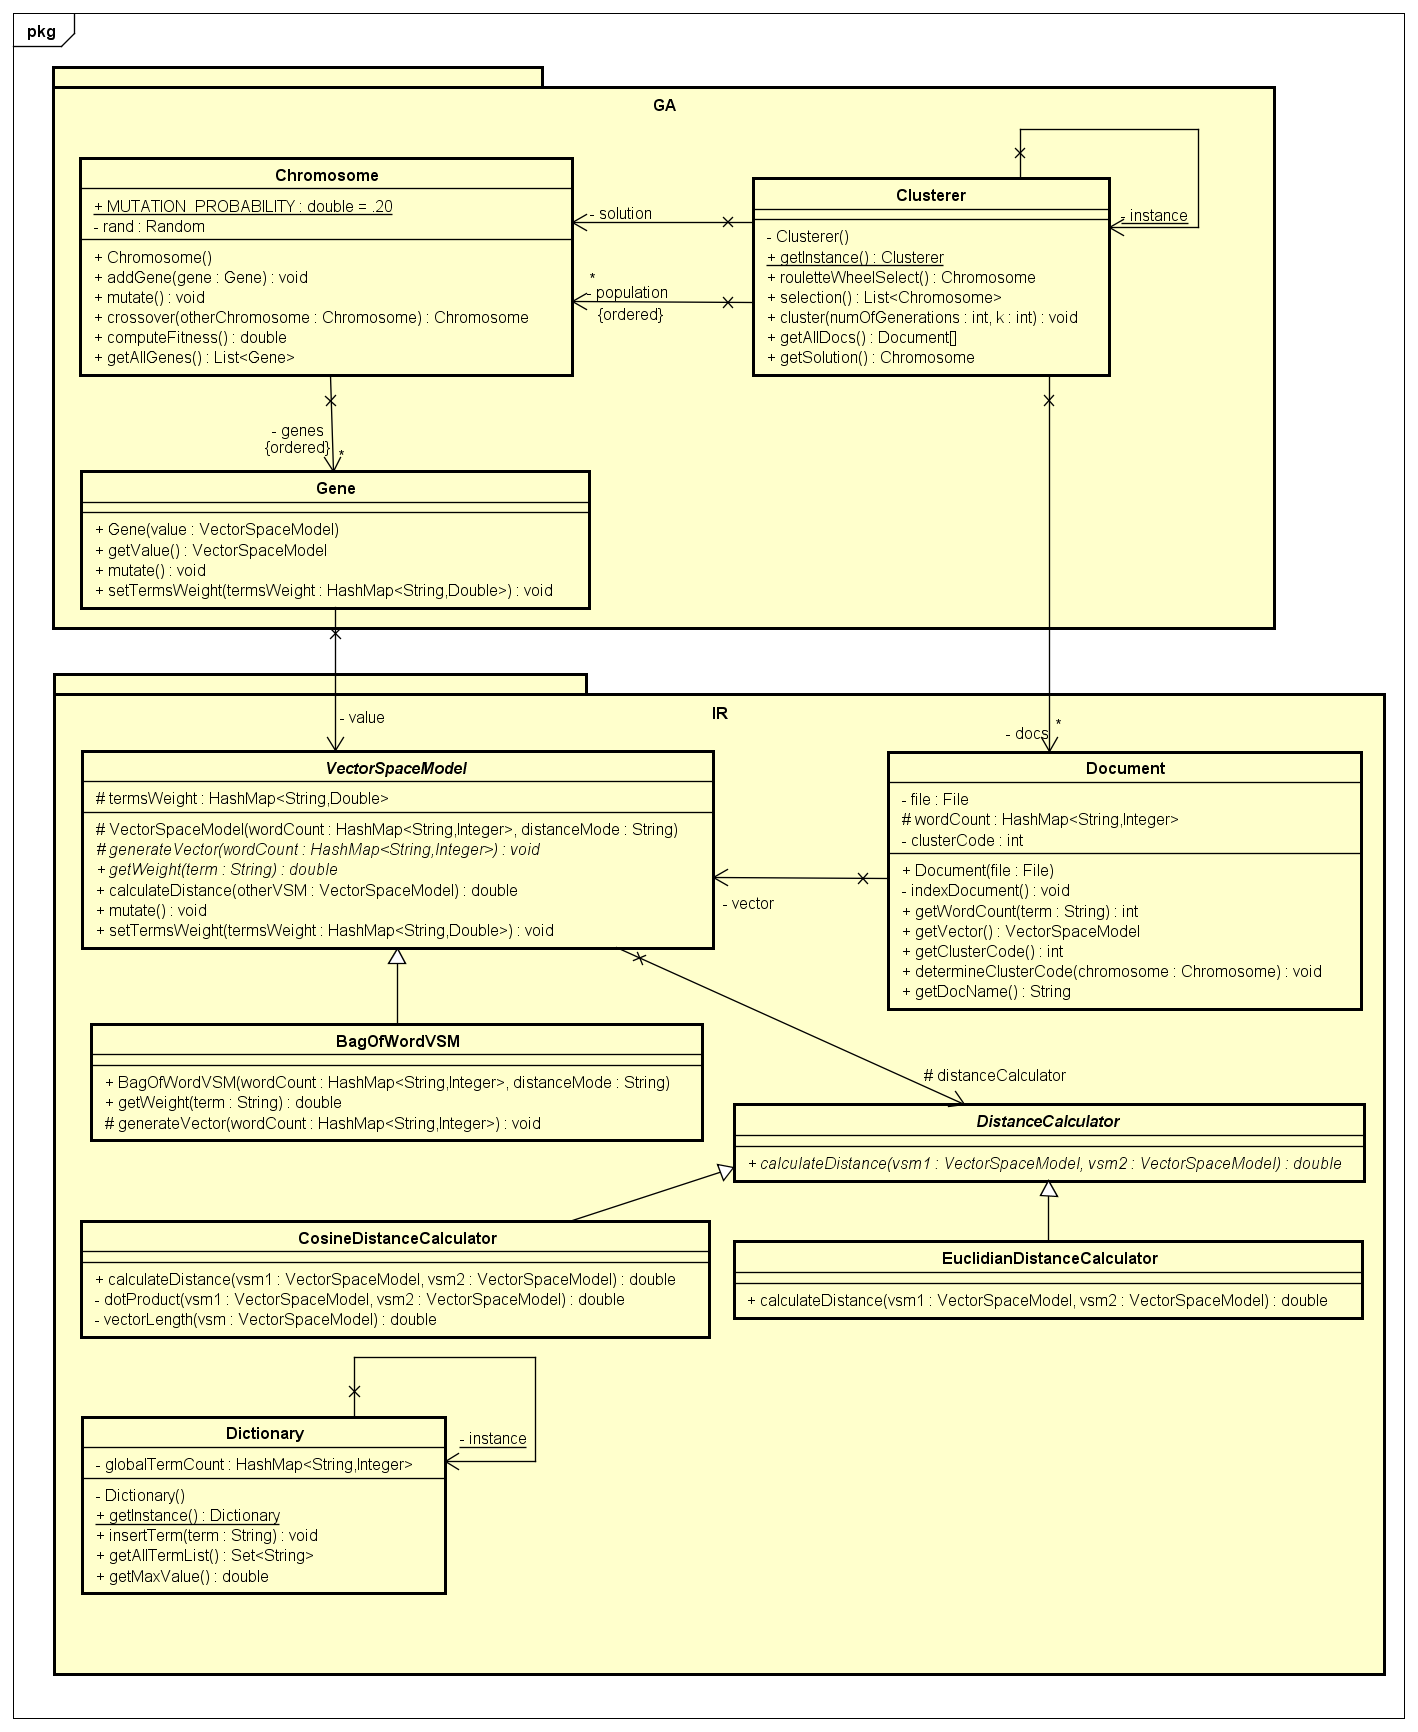
\includegraphics[width=\textwidth]{DiagramKelas}
%		\caption{\textit{Diagram Kelas}}
%		\label{fig:diagramkelas}
%	\end{center}
%\end{figure}